\begin{frame}
	\frametitle{Curve Ellittiche}

\begin{columns}
	\begin{column}{.65\textwidth}

		\begin{itemize}
			\item varietà abeliane 
			\item curve algebriche piane definite da: $y^2=x^3+ax+b$
			\item non singolari: $4a^3+27b^2\neq 0$
		\end{itemize}

		\begin{theorem}[Hasse]
			 sia $\mathbb{F}_q$ il campo di Galois di ordine $q$ 
			 \newline sia $\mathcal{E}=\mathcal{E}_{(a,b)}(\mathbb{F}_q)$ una curva ellittica su $\mathbb{F}_q$ 
			\vspace*{4pt}
			\begin{enumerate}
				\item $|o(\mathcal{E})-(q+1)|\leq2\sqrt q$
			\end{enumerate}	
		\end{theorem} 
		$\;\;\;\Rightarrow\;\;$l'ordine del campo finito usato governa la \textit{difficoltà}

	\end{column}

	\begin{column}{.4\textwidth}
		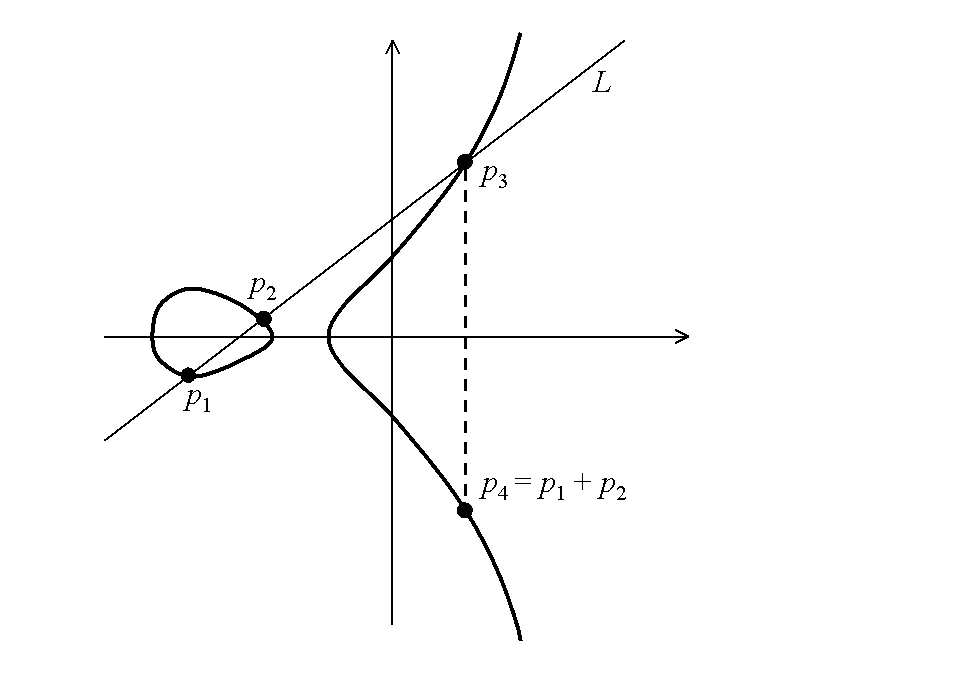
\includegraphics[height = 5 cm]{images/eca.png}
	\end{column}
\end{columns}

\end{frame}
%-------------------------------------------------------------------------
\begin{frame}
	\frametitle{Curve Ellittiche}
	\framesubtitle{legge di gruppo}
	
	$$ R= P+Q \triangleq(x_R,-y_R): $$ %SAY definisco operatore +
			  $$\left \{ \begin{array}{lr}
			  
			  				y_R=y_P+s(x_R-y_P) \\

							x_R = \left\{
								  \begin{array}{lcr}
								    s^2-2x_P & s=\frac{3x_P^2-p}{2y_P} &: x_P = x_Q \\
								    s^2-x_P-x_Q & s=\frac{y_P-y_Q}{x_P-x_Q} &\text{else}
								  \end{array}
								\right.
						\end{array} \right. $$
 	\vspace{1pt}				
 	$$ R = P\times n \triangleq P+P+\ldots+P\;\;\;\;\;\;\;\;\; n\;\mathrm{volte}$$
	\begin{figure}[H]
	 	\begin{center}
			 \begin{tabular}{c @{\hspace{1em}} c}
				 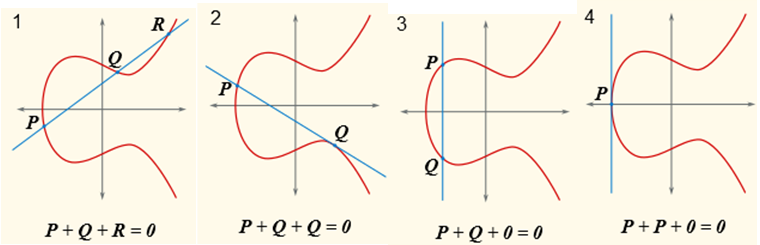
\includegraphics[height = 3 cm]{images/ecalgebrarow.png}
			 \end{tabular}
		 \end{center}
 	\end{figure}
	
\end{frame}
%-------------------------------------------------------------------------
\begin{frame}
	\frametitle{Curve Ellittiche}
	\framesubtitle{problema matematico}
	
	$(\mathcal{E}_{(a,b)}(\mathbb{F}_q),\,+)$ è un gruppo abeliano
	\begin{itemize}
		\item chiusura
		\item associatività
		\item identità %SAY come visto prima
		\item invertibilità %SAY come visto prima
		\item commutatività
	\end{itemize}  
	
	{\color{blue}Problema}: trovare ${\color{red}d}\in[1,\,n-1]$, dati
	\begin{itemize}
	  \item $\orange{\mathcal{E}}=\mathcal{E}_{(a,b)}(\mathbb{F}_q)$
	  \item $\orange{G}\in \mathcal{E}:\;\;\;\;\;\;\tiny{<}\,G\,\tiny{>}=\mathcal{E}$
	  \item $\orange{n}=o(G):\;G\times n= O=P_\infty$, $n$ primo
	  \item $\orange{P}\in \mathcal{E}$
	  \item $\orange{Q}=P\times d$
	\end{itemize}
\end{frame}